%%%% CONCLUSIONS %%%%
\chapter{Conclusions}\label{chap:11_Conclusions}
% Summary of contributions

In this thesis, we have explored the problem of, and state-of-the-art methods for, virtual navigation of ambisonics-encoded sound fields, with a particular emphasis on the challenges and perceptual penalties related to the region of validity restriction.%
\footnote{Recall that the region of validity restriction states that the spherical-harmonic description of a sound field, as captured by an ambisonics microphone, is only valid in a spherical region around the microphone that extends up to the nearest source or scattering body, i.e., only in the free-field.
See \secref{sec:02_Acoustical_Theory:Helmholtz_Equation} for more details.}
The primary contributions comprising this work can be summarized as follows:
\begin{itemize}
\item we have proposed, for the purpose of evaluating and comparing navigational methods, a suite of perceptually-relevant objective metrics and models for sound level, spectral coloration, perceived localization, and diffuseness (as enumerated in \secref{sec:06_Simulation_Framework:Metrics} and defined in \chapreftwo{chap:04_Auditory_Models}{chap:05_Proposed_Models});
\item in particular, we have developed, and subsequently validated through subjective listening experiments, auditory models for perceived localization and coloration (see \chapref{chap:05_Proposed_Models});
\item we have implemented and experimentally validated a numerical simulation framework with which one can comprehensively characterize the performance of a given navigational method (see \chapreftwo{chap:06_Simulation_Framework}{chap:10_Experimental_Validation});
\item we have provided critical reviews of existing extrapolation- and interpolation-based navigational methods (see \secreftwo{sec:07_Characterization_Extrapolation:Introduction}{sec:08_Proposed_Method:Introduction}, respectively), through which we have identified a number of common issues facing those methods;
\item we have characterized and compared the performance of linear extrapolation methods (see \chapref{chap:07_Characterization_Extrapolation}) as well as linear and parametric interpolation methods (see \chapreftwo{chap:08_Proposed_Method}{chap:09_Thiergart_Comparison});
\item through these evaluations, we have explored the particular penalties associated with violating the region of validity restriction (see \chapreftwo{chap:07_Characterization_Extrapolation}{chap:08_Proposed_Method});
\item we have proposed a parametric interpolation method which ensures that this restriction is not violated (see \chapref{chap:08_Proposed_Method}); and
\item we have identified practical guidelines with which future researchers might choose between the parametric navigational methods considered here, depending on their intended application (see \chapref{chap:09_Thiergart_Comparison}).
\end{itemize}
In this final chapter, we summarize the major findings that have resulted from this work, synthesize our earlier findings related to violating the region of validity restriction into broader insights, identify additional practical guidelines with which to choose between all of the methods considered here, and finally propose some possible avenues for further research.

\section{Summary of major findings}
Below, we summarize the four major findings that have resulted from this work.

%% Ch 5 - new models
\paragraph{Perceived localization and coloration can be accurately predicted directly from ambisonics impulse responses.}
In \chapref{chap:05_Proposed_Models}, we developed auditory models to predict, from an ambisonics impulse response, the perceived localization of a source and the perceived spectral coloration compared to a reference signal.
Traditionally, these attributes are estimated using binaural models, the predictions of which are necessarily confounded by the adopted ambisonics-to-binaural rendering approach.
Our proposed localization model extends the precedence-effect-based energy vector model of \citet{Stitt2016} by providing a pre-processing front end that extracts, from the ambisonics impulse response, a finite set of spatially- and temporally-distinct ``wavelets,'' all of which are then fed into the energy vector model in order to compute a single perceived source direction (see \secref{sec:05_Proposed_Models:Localization_Model} for more details).
%Our model essentially consists of that model and a pre-processing front end, which breaks the ambisonics impulse response into a finite set of discrete sounds with directions-of-arrival given by a plane-wave decomposition, times-of-arrival found by splitting each plane-wave impulse response into distinct ``wavelets'' identified via thresholding, and signal amplitudes given by a gammatone filter bank applied to each wavelet (see \secref{sec:05_Proposed_Models:Localization_Model} for more details).
We validated our model through a comparison with the results of a subjective localization experiment, in which subjects were asked to judge source directions for a set of measured and interpolated ambisonics impulse responses (rendered binaurally with head-tracking).
This comparison revealed 1) that our model performs comparably, if not superior, to the well-established binaural localization model of \citet{Dietz2011} and 2) that the \textit{structure} of our model is indeed valid, as the model was able to achieve (after optimizing its free parameters using the data) an average prediction error of only $3.67^\circ$ and a correlation coefficient between the predictions and data of $0.85$.

Our coloration model comprised a linear combination of two distinct metrics of spectral distortion: the range (in dB) of the difference spectrum after critical-band filtering (see \secref{sec:04_Auditory_Models:Coloration_Metrics:ABSE}) and the average depth of narrowband notches (see \secref{sec:04_Auditory_Models:Coloration_Metrics:Epk}).
We validated this model through a comparison with the results of a subjective coloration experiment, in which subjects were asked to rate spectral differences between modified and reference ambisonics impulse responses (rendered binaurally).
This comparison revealed that the two metrics included in the model are both dominant factors in human perception of coloration, such that each may serve independently as a useful measure of perceptible spectral coloration.

%% Ch 7 - extrapolation errors
\paragraph{Level and localization performance of linear extrapolation methods degrades for near-field sources.}
In \chapref{chap:07_Characterization_Extrapolation}, we characterized and compared, through numerical simulations and in terms of our proposed suite of objective metrics, the performance of two linear extrapolation methods: plane-wave translation and ambisonics translation (reviewed in \secreftwo{sec:03_Navigation_Techniques:PW_Technique}{sec:03_Navigation_Techniques:SR_Technique}, respectively).
An analysis of the plane-wave translation method alone revealed a clear advantage to matching the number of plane-wave terms, when computed via the ``beamforming'' plane-wave decomposition method, to the number of ambisonics signals.

With this implementation, the plane-wave translation method was shown to accurately reproduce both the level and localization of far-field sources.
In contrast, the ambisonics translation method was shown to incur significant errors in both level and coloration, which increase steadily with translation distance, due primarily to the low-pass-like roll-off of high-frequency energy seen in the frequency response induced by the method (see \figref{fig:07_Characterization_Extrapolation:Azimuth_Dependence:SRE}, for example).
In our analysis, we also showed that the performance of both methods degrades for near-field sources, since such sources lead to violations of the region of validity restriction.
In particular, when reproducing a near-field source, both methods incurred significant localization errors as well as a deficiency in the reproduced sound level.

%% Ch 8 - proposed method
\paragraph{Parametric exclusion of invalid microphones improves coloration performance and localization accuracy.}
In \chapref{chap:08_Proposed_Method}, we characterized and compared the performance of our proposed parametric interpolation method to that of a benchmark linear interpolation method.
Our method ensures, using the known or inferred positions of any near-field sources, that the region of validity restriction is not violated by excluding from the interpolation calculation those microphones that do not provide a valid description of the sound field at the position of the listener.
In contrast, the benchmark method simply computes a per-channel weighted-average across the microphones, with weights determined by the position of the listener (see \secref{sec:03_Navigation_Techniques:XF_Technique} for more details).

Through our analysis, we showed that the benchmark method introduces 1) large localization errors for near-field sources due to the precedence effect imposed by the nearest microphone to the source, 2) significant spectral errors due to comb-filtering, and 3) excessive diffuseness due to conflicting localization information between the two microphones.
The proposed method, on the other hand, achieves significantly improved localization performance, smaller spectral errors, and virtually exact diffuseness, all as a consequence of excluding the invalid microphone.

%% Ch 9 - time-frequency method
\paragraph{The time-frequency analysis method improves localization but degrades coloration performance in applications with a sparse microphone array and intimate sources.}
In \chapref{chap:09_Thiergart_Comparison}, we compared the parametric time-frequency interpolation method of \citet{Thiergart2013} to our proposed parametric method and, using trends observed in the data, we presented practical guidelines with which to choose between the two methods.
In order to distinguish between various potential applications, we first defined three practically-relevant ``axes'': the sparsity of the microphone array, the intimacy (i.e., proximity) of the sound sources, and the complexity of the sound field (see \secref{sec:09_Thiergart_Comparison:Conclusions} for definitions of these terms).
For applications spanning the first two axes, we also determined domains over which each method yields \textit{accurate and superior} performance, compared to the other method, in terms of spectral coloration and localization accuracy (see \figref{fig:09_Thiergart_Comparison:Region_Plots} and corresponding text).
%First, the \textit{sparsity} of the microphone array compares the size of the desired navigable region to the number of ambisonics microphones available. % u and \Delta/2 for P = 1,2
%Second, the \textit{intimacy} of the sound sources compares the average source distance (from the origin) to the size of the microphone array (or the size of the navigable region for a single microphone). % 1/\gamma
%Finally, the \textit{complexity} of the sound field refers to the number of sources and reflecting surfaces in the sound field.

According to the results of our analysis, for most applications with a sparse microphone array and with intimate sources, the time-frequency method will achieve superior localization performance, whereas the proposed method will incur less spectral coloration.
Additionally, for intimate sources, the time-frequency method will likely better convey source distance information due its accurate reproduction of sound level (which is a dominant cue in human perception of source distance \citep[section 3.1.1]{Zahorik2005}).%
\footnote{This potential benefit may be negated by the coloration introduced by the time-frequency method (see \figref{fig:09_Thiergart_Comparison:Spectral_Errors:Thiergart}), since spectrum is also a dominant perceptual cue for source distance \citep[section 3.1.3]{Zahorik2005}.
However, while the relationship between level and perceived distance is rather straightforward, the relationship between coloration and distance is less so, since only certain types of coloration (e.g., a high-shelf-like filter mimicking atmospheric absorption) are likely to influence perceived distance.}
For distant sources, on the other hand, the proposed method offers a marginal improvement over the time-frequency method in both spectral coloration and source localization.
Finally, the time-frequency method is likely preferable for acoustically simple sound fields, as it will yield superior localization accuracy and since its deficiency in diffuseness may not be noticeable, whereas, for acoustically complex sound fields, the proposed method is likely preferable due to its accurate reproduction of diffuseness.

\section{Penalties related to the region of validity}
% From Ch. 1 objectives: we seek broader insights into the nature of the penalties incurred by violating the region of validity restriction

In \chapreftwo{chap:07_Characterization_Extrapolation}{chap:08_Proposed_Method}, we drew separate insights for extrapolation and interpolation methods, respectively, regarding the penalties incurred by violating the region of validity restriction.
Here, we synthesize these findings into broader insights on this subject.

% bad localization due to drastic changes in direction geometry
First, we note that, in the presence of a near-field source, both extrapolation methods as well as the weighted-average interpolation method exhibit extremely large localization errors ($e_\nu > 30^\circ$) for translation distances larger than approximately $0.5$~m (see \figrefthree{fig:07_Characterization_Extrapolation:Localization_Errors:PWT}{fig:07_Characterization_Extrapolation:Localization_Errors:SRE}{fig:08_Proposed_Method:Localization_Errors:XF}).
This is primarily a geometric effect: as the listener traverses the navigable region (as defined in \secref{sec:06_Simulation_Framework:Geometry} for both the extrapolation and interpolation geometries), the intended source direction can change drastically, in particular when comparing listener positions inside and outside of the region of validity.
Evidently, none of these linear methods (extrapolation and weighted-average interpolation) can adequately compensate for the changing intended direction of the source as the listener moves.
However, both of the parametric interpolation methods considered in this thesis ensure, by construction, that the region of validity restriction is not violated and, consequently, they both achieve significantly improved localization errors under the same conditions (see \figref{fig:09_Thiergart_Comparison:Localization_Errors}).

% excessive diffuseness for interpolation methods due to conflicting localization information
A related error exhibited by the weighted-average interpolation method is the excessive diffuseness in the reproduced sound due to the conflicting localization information captured by the microphones for a near-field source (see \figref{fig:08_Proposed_Method:Diffuseness_Errors:XF}).
Although the extrapolation methods do not exhibit this error, we expect that any other interpolation method that does not compensate for the conflicting localization information will suffer from this error as well.

% bad levels due to drastic changes in distance geometry
Another common error introduced when the region of validity restriction is violated is that the reproduced sound level is several dB too low (see \figrefthree{fig:07_Characterization_Extrapolation:Level_Errors:PWT}{fig:07_Characterization_Extrapolation:Level_Errors:SRE}{fig:08_Proposed_Method:Level_Errors:XF}).
This too is largely a geometric effect, since none of the linear methods considered here are able to adequately increase the reproduced level as the listener navigates very close to a source.
Indeed, even our proposed method, which ensures that the region of validity restriction is not violated, exhibits a very similar error (see \figref{fig:08_Proposed_Method:Level_Errors:Hybrid}) since it does not amplify the microphone signals as the listener approaches a source.
Only the parametric time-frequency method (described in \secref{sec:03_Navigation_Techniques:Thiergart_Method}), which models the sound field with a virtual point source at the estimated position of the real source, is able to adequately reproduce the sound levels of near-field sources (see \figref{fig:09_Thiergart_Comparison:Level_Errors:Thiergart}).

% summarize
In sum, the penalties introduced by violating the region of validity restriction relate primarily to the drastic changes in the apparent geometry of the sound field as the listener navigates.
In particular, methods that do not account for the region of validity restriction are unable to adequately reproduce for near-field sources both the level changes due to longitudinal translations (i.e., towards or away from the source) and the localization changes due to lateral translations (perpendicular to the direction of the source).
Additionally, for interpolation methods that do not account for the region of validity restriction, the conflicting apparent geometries captured by the different microphones will incur not only degraded localization accuracy but also an excessive diffuseness in the reproduced sound.

\section{Practical implications}
% From Ch. 1 objectives: we identify considerations regarding the suitability of each method to various applications

In \secref{sec:09_Thiergart_Comparison:Conclusions}, we identified several general principles with which to choose between the two parametric interpolation methods considered in that chapter for various potential applications.
As mentioned above, we discussed these applications in terms of three axes: the sparsity of the microphone array, the intimacy of the sound sources, and the complexity of the sound field. % (see \figref{fig:09_Thiergart_Comparison:Practical_Axes}).
Building on that discussion, here, we identify several additional principles for choosing between all of the methods considered in this work:
\begin{enumerate}
% sparsity axis
\item[1a.] With a sparse microphone array, the weighted-average method will achieve a marginal improvement in spectral coloration over the time-frequency method.
The ambisonics translation method should be avoided as it will incur significant level and spectral errors for even a moderately-sized (e.g., $\sim0.5$~m) navigable region.
\item[1b.] With a dense microphone array, the weighted-average method will yield the smallest localization errors, although none of the methods considered here will achieve particularly accurate localization unless the sources are very far away.
%This is an area for future development.
% intimacy axis
\item[2a.] When recording primarily intimate sources, all of the linear methods will incur significant localization errors and the weighted-average method in particular will introduce excessive diffuseness.
\item[2b.] When recording primarily distant sources, the plane-wave translation method will yield accurate reproductions of sound level, localization, and diffuseness with just a single ambisonics microphone.
The weighted-average method will yield similarly accurate reproductions of these metrics.
% complexity axis
\item[3a.] For an acoustically complex sound field, the linear methods may be advantageous since 1) by construction, they can trivially accommodate multiple sources and 2) the extrapolation methods will accurately reproduce diffuseness, and the additional diffuseness introduced by the weighted-average method for intimate sources may not be noticeable.
\item[3b.] For an acoustically simple sound field, however, the excessive diffuseness introduced by the weighted-average method for near-field sources may be particularly distracting.
\end{enumerate}

As an extension of the analysis presented in \secref{sec:09_Thiergart_Comparison:Conclusions} (and summarized above), here we determine, for all of the methods considered in this thesis, the domains (across array sparsity and source intimacy and in terms of coloration and localization) over which each method yields both \textit{accurate and superior} performance, where we define ``accurate'' performance as achieving spectral errors of $\rho_\eta < 3$~dB and localization errors of $e_\nu < 10^\circ$.
These domains are sketched in \figref{fig:11_Conclusions:Region_Plots}.

\begin{figure*}[t]
	\centering
	\begin{subfigure}[b]{0.49\textwidth}
		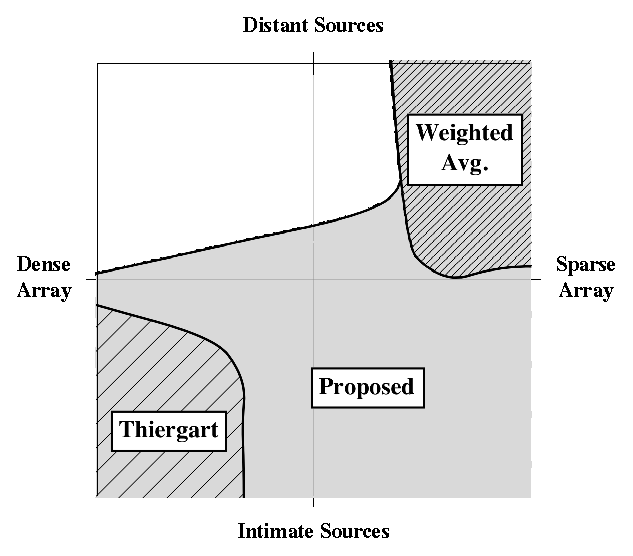
\includegraphics[width=\textwidth]{11_conclusions/figures/Coloration_Region_Plot}
		\caption{Coloration}
		\label{fig:11_Conclusions:Region_Plots:Coloration}
	\end{subfigure}
	\hfill
	\begin{subfigure}[b]{0.49\textwidth}
		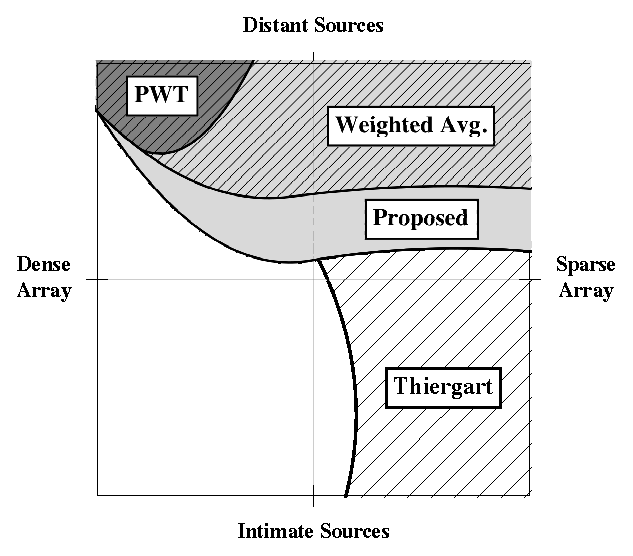
\includegraphics[width=\textwidth]{11_conclusions/figures/Localization_Region_Plot}
		\caption{Localization}
		\label{fig:11_Conclusions:Region_Plots:Localization}
	\end{subfigure}
	
	\caption[Region plots of practical applicability of each navigational method.]{
	Region plots illustrating accurate and superior methods in terms of spectral coloration (left panel) and localization accuracy (right) across practical applications with varying microphone array sparsity (horizontal axis) and sound source intimacy (vertical).
	The gray filled regions correspond to the proposed method;
	the coarsely-hatched regions correspond to the time-frequency method of \citet{Thiergart2013};
	the finely-hatched regions correspond to the weighted-average interpolation method;
	and the dark gray filled region corresponds the plane-wave translation method (labeled ``PWT''), in addition to the proposed method.
	Regions that are both filled and hatched indicate that the methods perform comparably;
	empty regions indicate that none of the methods satisfy the specified error limit.}
	\label{fig:11_Conclusions:Region_Plots}
\end{figure*}

From \figref{fig:11_Conclusions:Region_Plots:Coloration}, we first note that no method offers any domain of accurate coloration performance that is distinct from that of the proposed method.
(Note that neither of the extrapolation methods offer sufficiently accurate coloration performance to appear in that plot.)
Furthermore, for localization (see \figref{fig:11_Conclusions:Region_Plots:Localization}), we see that the regions of accurate performance for the two linear methods shown are contained within that of the proposed method.
Only the time-frequency method offers a distinct (from the proposed method) practical domain of accurate localization performance: in applications with a sparse microphone array and intimate sources.

From these figures, we also note that the weighted average method, similarly to the proposed method, offers accurate performance in both coloration and localization in applications with a sparse microphone array and distant sources.
This is unsurprising, since for distant sources (i.e., since the region of validity is not violated), the proposed method performs a very similar interpolation calculation to that done by the weighted average method (see \secref{sec:08_Proposed_Method:Hybrid_Technique}).

% some more general results across methods, not necessarily along the axes
Of all of the methods considered in this thesis, either of the parametric interpolation methods is generally preferable over any of the linear methods for most applications, since, except where noted above, the parametric methods tend to outperform the linear ones.
In particular, in most applications, both of the parametric methods considered here achieve significantly improved localization accuracy compared to the linear methods.
The results presented in this thesis also show that any interpolation method will yield significantly improved spectral errors compared to either of the extrapolation methods.

% some sort of concluding thing
It should be emphasized that the existing body of literature relating to virtual navigation of ambisonics-encoded sound fields has been largely numerical in nature (and the present thesis is no exception), so this particular field of research is notably lacking in practical experience.
Consequently, it is our hope that the guidelines enumerated above (as well as those in \secref{sec:09_Thiergart_Comparison:Conclusions}) will facilitate more real-world implementations of the navigational methods considered in this thesis.
Ideally, future experimental investigations and subjective assessments of these (and other) methods will further illuminate the deficiencies of the existing methods and thereby inform the development of novel ones.

\section{Future work}
% explore different sound fields / source configurations
The analyses presented in this thesis provide a baseline set of characterizations of the various navigational methods considered here.
One avenue for further research is to consider additional types of simulated sound fields, such as those consisting of multiple sources, directional sources, and/or reflective surfaces.
Parametric methods in particular warrant additional analyses to establish their performance in the presence of multiple sources, which may cause deviations from the results published here.
Furthermore, in immersive applications with intimate sources, the ability of a navigational method to accurately capture and reproduce the directivities of those sources may be critical, but this issue is largely unexplored in the literature (with the exception of the study by \citet{Wakayama2017}).
%Since, by construction, the time-frequency method models the incident sound field as a collection of omnidirectional point sources, it might be expected that this method will be unable to accurately reproduce any other directivity.

% explore different methods / microphone configurations
Additionally, in the present thesis, we considered only a subset of all existing navigational methods (see \tabref{tab:01_Introduction:Methods}).
Future investigations should therefore consider alternative methods, such as the parametric extrapolation methods of \citet{Wakayama2017} and \citet{Plinge2018}, which, like the parametric interpolation methods considered in this thesis, should be able to circumvent the region of validity restriction.
One might also extend the characterizations of the interpolation methods considered here to two-dimensional array configurations, such as an equilateral triangle or a square (cf.~\citet{Mariette2010} and \citet{Bates2018}, respectively).

% explore additional metrics / models
Future research might also seek to enlarge or improve the set of objective auditory metrics and models which we have employed throughout this thesis.
For example, although errors in the reproduced sound level are likely sufficient to produce errors in distance perception \citep[section 3.1.1]{Zahorik2005}, it may be useful to develop a dedicated model for perceived source distance, perhaps based on the known formula for distance coding of point-sources (see \eqnref{eq:02_Acoustical_Theory:PointSource_An}).
Additionally, subjective evaluations of stimuli with varying diffuseness should be conducted in order to establish a perceptual threshold for audibility of diffuseness errors.

% sensitivity analysis
Finally, although we have endeavored to make the analyses presented in this thesis practically relevant, we did not consider any sensitivities of the navigational methods to small errors that may arise in practice.
Consequently, any degradations in performance incurred due to errors in microphone placement or orientation should be quantified.
Additionally, as both of the parametric methods considered here require estimates of the positions of sources, the impact of any estimation errors (e.g., triangulation errors due to noise) on the performance of those methods should be explored.